\documentclass{article}
\usepackage{amsmath}
\usepackage{amssymb}
\usepackage{graphicx}
\usepackage{hyperref}
\usepackage[version=4]{mhchem}


\begin{document}
\(D A\) and \(D B\) are tangent to circle \(O\) at \(A\) and \(B\), respectively. \(A C\) is the diameter of circle \(O\). Prove: \(\angle A D B=2 \angle B A C\).

Solution:
Connect \(B C\).\\
\centering
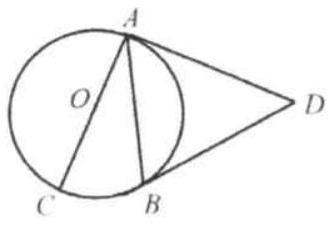
\includegraphics[width=\textwidth]{images/163(2).jpg}

Since \(A C\) is the diameter, \(\angle A B C=90^{\circ}\).\\
\(\angle C A B+\angle A C B=\alpha+\beta=180^{\circ}-90^{\circ}=90^{\circ}\).\\
\(\angle A C B=\angle B A D\) (both face the same arc \(A B\) ).\\
So \(\angle B A D=\beta\).\\
Note that \(\triangle D A B\) is an isosceles triangle, \(\angle D B A=\beta\).\\
\centering
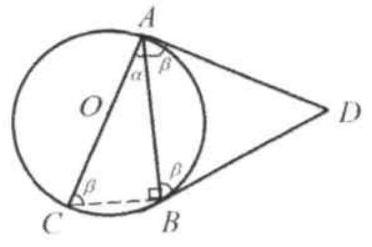
\includegraphics[width=\textwidth]{images/163(4).jpg}

Thus \(\alpha=90^{\circ}-\beta \quad \Rightarrow \quad 2 \alpha=180^{\circ}-2 \beta\)\\
In triangle \(A D B, \angle A D B=180^{\circ}-2 \beta=2 \alpha=2 \angle B A C\).


\end{document}
